\subsection*{Partie 1. Nature des trajectoires}
\begin{figure}
 \centering
 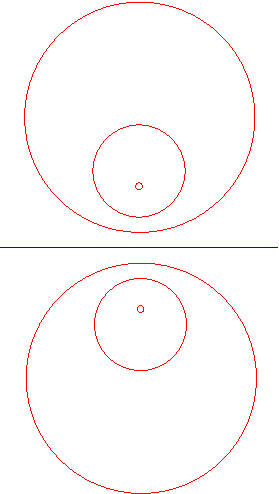
\includegraphics{Cricatti_1.pdf}
 % Cricatti_1.pdf: 226x400 pixel, 72dpi, 7.97x14.11 cm, bb=0 0 226 400
 \caption{Trajectoires de $z'=1+z^2$.}
 \label{fig:Cricatti_1}
\end{figure}
\begin{enumerate}
 \item Si $v$ est la valeur complexe d'une fonction constante solution de l'éqation différentielle, elle doit vérifier
\begin{displaymath}
 1+v^2 = 0
\end{displaymath}
 On en déduit qu'il existe deux solutions constantes, elles ont pour valeur $+i$ et $-i$.
\item La restriction à $]-\frac{\pi}{2},+\frac{\pi}{2}[$ de la fonction $\tan$ est solution de l'équation $(1)$.
\item En séparant les parties réelles et imaginaires, on obtient le système 
\begin{displaymath}
 (\mathcal S)
\left\lbrace
\begin{aligned}
 x' &= 1+x^2-y^2 \\
 y' &= 2xy
\end{aligned}
 \right. 
\end{displaymath}
\item On utilise encore les notations $x$ et $y$ de la question précédente.
\begin{displaymath}
 \left(\frac{y}{1+x^2+y^2}\right)^\prime
=\frac{y'}{1+x^2+y^2} - \frac{2y(xx'+yy')}{(1+x^2+y^2)^2}
\end{displaymath}
En multipliant les lignes de $(\mathcal S)$ par $x$ et $y$, on obtient:
\begin{displaymath}
 xx'+yy' =x+x^3+xy^2=x(1+x^2+y^2)
\Rightarrow
\left(\frac{y}{1+x^2+y^2}\right)^\prime = 0
\end{displaymath}

\item Dans la question précédente, on a montré qu'une certaine expression était constante. Prenons sa valeur en $0$.
\begin{multline*}
 \frac{y(t)}{1+x^(t)+y^(t)}=\frac{\lambda}{1+\lambda^2}
\Leftrightarrow x^2(t)-\left(\lambda + \frac{1}{\lambda} \right)y(t)+y^2(t)=-1\\
\Leftrightarrow x^2(t)+\left(y(t)-\frac{1}{2}(\lambda + \frac{1}{\lambda}) \right)^2= -1 + \frac{1}{4}(\lambda + \frac{1}{\lambda})^2 = \frac{1}{2}(\lambda - \frac{1}{\lambda})^2
\end{multline*}
On en déduit que la trajectoire est incluse dans le cercle :
\begin{align*}
 \text{coordonnées du centre : } \left( 0,\frac{1}{2}(\lambda + \frac{1}{\lambda}) \right) & &
\text{rayon : } \frac{1}{2} \left\vert \lambda - \frac{1}{\lambda}\right\vert
\end{align*}
La figure \ref{fig:Cricatti_1} présente le tracé de quelques trajectoires pour des valeurs de $\lambda$. Les points d'intersection avec l'axe $(Oy)$ ont pour ordonnées :
\begin{displaymath}
 \frac{1}{2}\left( \lambda + \frac{1}{\lambda}\right)  \pm \frac{1}{2} \left( \lambda - \frac{1}{\lambda}\right)
= \lambda \text{ ou } \frac{1}{\lambda}
\end{displaymath}
\end{enumerate}

\subsection*{Partie 2. Expressions des solutions.}
\begin{enumerate}
 \item\begin{enumerate}
 \item Les solutions sont de la forme $t\rightarrow\lambda e^{A(t)}$ où $\lambda\in \C$ et $A$ une primitive de $t\rightarrow2\tan t$.\\
Dans l'intervalle $]-\frac{\pi}{2},\frac{\pi}{2}[$, le $\cos$ est strictement positif. On peut choisir $A(t)=\ln(\cos(t))$. Les solutions sont donc les fonctions
\begin{displaymath}
 \forall t \in ]-\frac{\pi}{2},\frac{\pi}{2}[ : t\rightarrow\lambda \cos^2t \text{ avec } \lambda\in \C
\end{displaymath}

\item On utilise la méthode de variation des constantes. On cherche une solution particulière sous la forme $t\rightarrow\lambda(t)\cos^2t$. La fonction $\lambda$ doit vérifier
\begin{displaymath}
 \lambda'(t)\cos^2t=-1
\end{displaymath}
On peut donc choisir $\lambda(t)=-\tan t$ ce qui conduit à la solution particulière
\begin{displaymath}
 t\rightarrow -\tan t \cos^2t=-\sin t \cos t
\end{displaymath}
 Les solutions sont donc les fonctions
\begin{displaymath}
 \forall t \in ]-\frac{\pi}{2},\frac{\pi}{2}[ : t\rightarrow -\sin t \cos t + \lambda \cos^2t \text{ avec } \lambda\in \C
\end{displaymath}
\end{enumerate}
 
\item \begin{enumerate}
 \item Ici $z$ est une solution telle que $z(0)=i\lambda$ avec $\lambda$ réel non nul. D'après la question 4. de la première partie, on a (pour \emph{tous} les $t$ de $I$):
\begin{displaymath}
 \frac{\Im(z(t))}{1+|z(t)|^2}=\frac{\lambda}{1+\lambda^2}\neq 0
\end{displaymath}
On en déduit que, pour tous les $t$ dans $I$, $z(t)\notin\R$. En particulier, il ne peut pas être égal à $\tan t$.\\
On aurait pu aussi raisonner en terme de problème de Cauchy.
\item Notons $u(t)=\frac{1}{z(t)-\tan t}$. On a alors $z(t)-\tan t =\frac{1}{u(t)}$ et on peut déduire :
\begin{multline*}
 \left. 
\begin{aligned}
 z'(t)&=1+z^2(t)\\
 \tan't &= 1+\tan^2 t\\
(\frac{1}{u})' &= -\frac{u'(t)}{u^2(t)}
\end{aligned} 
\right\rbrace 
\Rightarrow z^2(t)-\tan^2t=  -\frac{u'(t)}{u^2(t)}\\
\Rightarrow \frac{z(t)+\tan t}{u(t)} =  -\frac{u'(t)}{u^2(t)} 
\Rightarrow \frac{2\tan t}{u(t)} + \frac{1}{u(t)^2} =   -\frac{u'(t)}{u^2(t)}\\
\Rightarrow u'(t)+2\tan(t)\, u(t) = -1
\end{multline*}
La fonction $u$ vérifie donc l'équation différentielle de la question 1.b.
\item D'après la question précédente et le résultat de la question 1.b, il existe un nombre complexe $\mu$ tel que :
\begin{displaymath}
 \forall t\in I : \frac{1}{z(t) -\tan t} = \mu \cos^2t-\sin t \cos t
\end{displaymath}
En prenant la valeur en $0$, on obtient $\mu=-\frac{i}{\lambda}$. On en déduit :
\begin{multline*}
 z(t)-\tan t = \frac{1}{-\frac{i}{\lambda}\cos^2t - \sin t \cos t} \\
\Rightarrow z(t)= \tan t - \frac{1+\tan^2t}{\tan t +\frac{i}{\lambda}} 
=\frac{\frac{i}{\lambda}\tan t -1}{\tan t +\frac{i}{\lambda}}=\frac{\tan t + \lambda i}{1-i\lambda \tan t}
\end{multline*}
\end{enumerate}
\item Dans cette question $z$ est une solution définie dans un intervalle $I$ contenant $0$ et telle que $z(0)=\lambda\neq0$.
\begin{enumerate}
\item La fonction $t\rightarrow z(t)-\tan t$ est continue en $0$ et elle prend en $0$ une valeur non nulle. Par continuité, il existe donc un intervalle $J$ dans lequel elle ne s'annule pas. Ici encore, on aurait pu raisonner en terme de problème de Cauchy. S'il existe un $t_0$ tel que $z(t_0)=\tan(t_0)$ alors les deux fonctions sont solutions d'une même problème de Cauchy en $t_0$ elles doivent donc coïncider dans leur domaine; en particulier en $0$ ce qui est contraire à l'hypothèse.\\
On peut considérer l'inverse dans $J$ de $z-\tan$.
\item Les calculs sont les mêmes qu'en 2.. La fonction indiquée vérifie l'équation différentielle de la question 1.b. Il existe un nombre complexe $\mu$ tel que
\begin{displaymath}
\forall t\in J : \frac{1}{z(t) -\tan t} = \mu \cos^2t-\sin t \cos t
\end{displaymath}
En prenant $t=0$, on obtient que $\mu=\frac{1}{\lambda}$ est réel et
\begin{multline*}
 z(t)-\tan t = \frac{1}{\frac{1}{\lambda}\cos^2t - \sin t \cos t} \\
\Rightarrow z(t)= \tan t + \frac{1+\tan^2t}{\frac{1}{\lambda}-\tan t } 
=\frac{\frac{1}{\lambda}\tan t +1}{\frac{1}{\lambda}-\tan t }=\frac{\tan t + \lambda}{1-\lambda \tan t}\\
=\tan(t+t_0) \text{ si } t_0=\arctan \lambda
\end{multline*}
On aurait aussi pu raisonner en \emph{séparant les variables}, lorsque $z$ est à valeurs réelles 
\begin{displaymath}
 \forall t\in J : \frac{z'(t)}{1+z^2(t)}=1\Rightarrow t\rightarrow \arctan(z(t))-t \text{ est constante.}
\end{displaymath}

\end{enumerate}
\end{enumerate}

\subsection*{Partie 3. Projection stéréographique.}
\begin{enumerate}
 \item 

\begin{enumerate}
\item Le seul point de la sphère pour lequel $\gamma=1$ est le pôle nord $N$ qui est exclu. En revanche $\alpha=\beta=0$ est aussi possible pour le pôle sud de coordonnées $(0,0,-1)$.\\
Lorsque $M\neq N$, on peut former une représentation paramétrique de la droite $(NM)$. Les coordonnées d'un point de cette droite sont de la forme $(\lambda\alpha,\lambda\beta,1+\lambda(\gamma-1))$ avec $\lambda$ réel. Un tel point est sur le plan si et seulement si
\begin{displaymath}
 1+\lambda(\gamma-1)=0\Leftrightarrow \lambda = \frac{1}{1-\gamma}
\end{displaymath}
On en déduit que l'affixe du projeté stéréographique est
\begin{displaymath}
 w=\frac{\alpha +i\beta}{1-\gamma}
\end{displaymath}
De plus, lorsque $(\alpha,\beta)\neq (0,0)$,
\begin{displaymath}
 w=w\frac{\alpha-i\beta}{\alpha-i\beta}=\frac{\alpha^2+\beta^2}{(1-\gamma)(\alpha-i\beta)}=\frac{1+\gamma}{\alpha-i\beta}
\end{displaymath}
car $\alpha^2+\beta^2+\gamma^2=1$ donc $\alpha^2+\beta^2=1-\gamma^2$.
\item D'après la question précédente :
\begin{displaymath}
 \left. 
\begin{aligned}
 w &= \frac{\alpha +i\beta}{1-\gamma}\\
 \overline{w}  &= \frac{\alpha +i\beta}{1-\gamma}
\end{aligned}
\right\rbrace 
\Rightarrow
\left\lbrace 
\begin{aligned}
 w+\overline{w} &=\frac{2\alpha}{1-\gamma}\\
w-\overline{w} &=\frac{2i\beta}{1-\gamma}
\end{aligned}
\right. 
\end{displaymath}
\begin{displaymath}
 |w|^2+1=\frac{\alpha^2+\beta^2}{(1-\gamma)^2}+1
=\frac{\alpha^2+\beta^2+1-2\gamma + \gamma^2}{(1-\gamma)^2}
=\frac{2(1-\gamma)}{(1-\gamma)^2}=\frac{2}{1-\gamma}
\end{displaymath}
On en déduit :
\begin{align*}
 \alpha = \frac{w+\overline{w}}{1+|w|^2} & & i\beta = \frac{w - \overline{w}}{1+|w|^2}
\end{align*}
On a aussi 
\begin{displaymath}
 1-\gamma=\frac{2}{|w|^2+1}\Rightarrow \gamma=1-\frac{2}{|w|^2+1}=\frac{|w|^2-1}{|w|^2+1}
\end{displaymath}

\item Il s'agit d'une petite question technique qui servira dans le calcul de la question 4.c. Avec les formules précédentes, on obtient 
\begin{align*}
 \frac{\gamma}{1-\gamma} &= \frac{|w|^2-1}{|w|^2+1}\frac{|w|^2+1}{2}=\frac{|w|^2-1}{2} \\
 \frac{\beta}{1-\gamma} &= \frac{i(\overline{w}-w)}{|w|^2+1}\frac{|w|^2+1}{2}=i\frac{\overline{w}-w}{2} 
\end{align*}
\end{enumerate}

\item Il s'agit ici d'utiliser les formules du cours permettant de dériver des fonctions formées à partir de produits scalaires. Les deux dérivées sont nulles car $\overrightarrow\Omega \wedge \overrightarrow{OM(t)}$ est orthogonal à $\overrightarrow\Omega$ et à $\overrightarrow{OM(t)}$.
\begin{align*}
 \frac{d}{dt}\left\Vert\overrightarrow{OM(t)}\right\Vert = 
\frac{(\overrightarrow{OM(t)}/\overrightarrow{M'}(t))}{\left\Vert\overrightarrow{OM(t)}\right\Vert} = 0  & &
\frac{d}{dt}(\overrightarrow\Omega/\overrightarrow{OM(t)}) =
(\overrightarrow\Omega/\overrightarrow{M'}(t))) = 0
\end{align*}
Le caractère constant  de $t\rightarrow \left\Vert\overrightarrow{OM(t)}\right\Vert$ montre que $M(t)$ reste sur une sphère centrée en $O$.\\
Le caractère constant  de $t\rightarrow (\overrightarrow\Omega/\overrightarrow{OM(t)})$ montre que $M(t)$ reste sur un plan orthogonal à $\overrightarrow\Omega$.\\
Le point $M(t)$ reste donc sur un cercle intersection d'une sphère et d'un plan.
\item Dans le repère choisi, seule la dernière coordonnée de $\overrightarrow \Omega$ est non nulle. On en déduit:
\begin{displaymath}
 \begin{pmatrix}
  0\\
0\\
\Vert \overrightarrow \Omega\Vert
 \end{pmatrix}
\wedge
\begin{pmatrix}
 X\\
Y\\
Z
\end{pmatrix}
=
\begin{pmatrix}
-\Vert \overrightarrow \Omega\Vert Y \\
\Vert \overrightarrow \Omega\Vert X\\
0
\end{pmatrix}
\Rightarrow
\left\lbrace 
\begin{aligned}
X'(t) &= -\Vert \overrightarrow \Omega\Vert Y(t)\\
Y'(t) &= \Vert \overrightarrow \Omega\Vert X(t)\\
Z'(t) &= 0
\end{aligned}
\right. 
\end{displaymath}

\item \begin{enumerate}
\item On dérive simplement l'expression de $w(t)$ obtenue en 1.a. en se dispensant d'écrire les $(t)$
\begin{displaymath}
 w'= \frac{\alpha'+i\beta'}{1-\gamma} + \underset{=w}{\underbrace{\frac{\alpha+i\beta}{1-\gamma}}}\frac{\gamma'}{1-\gamma}
= \frac{\alpha'+i\beta'+w\gamma'}{1-\gamma}
\end{displaymath}
\item On obtient la formule annoncée en injectant les expressions des dérivées
\begin{displaymath}
 \begin{pmatrix}
  \alpha'\\
\beta'\\
\gamma'
 \end{pmatrix}
=
\begin{pmatrix}
 p\\q\\r
\end{pmatrix}
\wedge
\begin{pmatrix}
 \alpha \\ \beta \\ \gamma
\end{pmatrix}
\end{displaymath}
dans la formule de la question précédente.
\item Divisons par $1-\gamma$ l'expression du 1.b. On obtient une expression de $w'$.
\begin{displaymath}
 w'(t)=
irw(t) + (q-ip)\frac{\gamma(t)}{1-\gamma(t)} -qw^2(t) +w(t)(p+iq)\frac{\beta(t)}{1-\gamma(t)}
\end{displaymath}
dans laquelle figurent les quantités calculées en 1.c. En développant, les $|w^2|$ disparaissent et on obtient
\begin{displaymath}
 w'(t) = irw(t)-\frac{1}{2}(q-ip)-qw^2(t) + \frac{1}{2}(q-ip)w^2
= a + bw(t) +cw^2(t)
\end{displaymath}
avec
\begin{align*}
 a=\frac{1}{2}(-q+ip) & & b=ir & & c=-\frac{1}{2}(q+ip)=\overline{a}
\end{align*}
On retrouve l'équation $(1)$ de la tangente pour $a=1$ et $b=0$ soit $p=0$, $q=-2$, $r=0$.
\end{enumerate}

\end{enumerate}

